%!TEX root = ../../main.tex
\toggletrue{image}
\toggletrue{imagehover}
\chapterimage{manage_your_preferences}
\chapterimagetitle{\uppercase{Manage Your Preferences}}
\chapterimageurl{\chapterimageurl{https://xkcd.com/2432/}}
\chapterimagehover{Manage cookies related to essential site functions, such as keeping Atrus and his sons imprisoned within the page.}

\chapter{Cookies mit \acs{PHP} setzen}
\label{chapter-cookies-php}

Kennen Sie das auch? Sie surfen zu einer Website und lesen \say{Schön, dass Sie uns \textbf{wieder} besuchen!}. Tatsächlich ist es nicht der erste Besuch. Noch nach Wochen \say{erinnert} sich ein Online-Shop an die Produkte, die Sie irgendwann mal zur Probe in den Warenkorb gelegt und nie gekauft haben. Manche Websites erinnern sich sogar noch nach Monaten an Ihren Namen und begrüssen Sie mit dem Benutzernamen (z.B. Amazon). Was steck dahinter? Hier handelt es sich aller Wahrscheinlichkeit nach um Cookies. Vor der \say{Erfindung} von Cookies war das Surfen im \ac{WWW} eine Reise ohne Geschichte und ist/wäre es auch heutzutage, wenn Cookies (oder ähnliche Techniken) unbekannt wären oder wenn Sie den Gebrauch im Browser deaktivieren (was Sie auch können).

\begin{definition}[Cookie]
Cookies sind \say{Informationskrümel}, die eine Webseite auf dem Computer des Benutzers speichert. Durch Cookies kann eine Website Textinformationen über den Benutzer speichern und sich an ihn \say{erinnern}. Meist werden sämtliche Cookies in einer Datei auf dem Rechner des Benutzers gespeichert. Das Speichern eines Cookies wird als \textbf{Cookie setzen} bezeichnet. Ruft ein Benutzer eine Website auf, dann schickt der Browser bereits gesetzte Cookie automatisch an den Webserver, damit dieser das Cookie auswerten kann.
\end{definition}

Die Lernziele lauten wie folgt:

\newcommand{\cookiesPhpLernziele}{
\protect\begin{todolist}
\item Sie erklären an einem Beispiel was man im \ac{WWW} unter einem Cookie versteht.
\item Sie informieren über die Eckdaten von Cookies und deren Sicherheitsbedenken.
\item Sie setzen mit \ac{PHP} ein Cookie und lesen es wieder aus.
%\item Sie erklären den Cookie-Scope.
\end{todolist}
}

\lernziel{\autoref{chapter-cookies-php}, \nameref{chapter-cookies-php}}{\protect\cookiesPhpLernziele}

\cookiesPhpLernziele

\section{Sind Cookies ein Sicherheitsrisiko?}

%https://makeameme.org/meme/cookies-cookies-everywhere-mid197

\begin{wrapfigure}[10]{r}{8cm}
\vspace{-\baselineskip}
\centering

\includegraphics[scale=0.5]{cookies_cookies_everywhere}
\end{wrapfigure}

Eigentlich nicht. Es kommt jedoch immer darauf an, wie der Webentwickler, diese Technologie einsetzt (damit sind auch Sie gemeint!). Meist haben Cookies im \ac{WWW} einen eher schlechten Ruf. Bei Surfern ist die Meinung weitverbreitet, dass über Cookies persönliche Daten aller Art weitergereicht werden. Prinzipiell ist es so, dass der Webserver nur Informationen in Cookies speichern kann, die ihm ohnehin schon bekannt sind und daher nur diese Informationen vom Browser wieder zurückgesandt bekommt. Sicherheitslücken von Browser können immer ein Problem darstellen, dies ist jedoch ein anderes Thema. Es gibt jedoch die Möglichkeit, Cookies zu missbrauchen. Wir könnten zum Beispiel das Surfverhalten von Usern \say{ausspionieren}. Eigentlich sind Cookies an eine Website gebunden. Das heisst, wir können nur das Surfverhalten pro Website analysieren. Es wurden jedoch Methoden entwickelt, die erlauben, Cookies von ausserhalb der besuchten Website zu setzen. Es handelt sich dabei um Cookies von Drittanbietern. Dies ist etwa möglich, wenn Sie ein externes Bild via Link auf Ihrer Website einbinden. In den meisten Browsern können Sie deshalb Cookies von Drittanbietern verbieten.

\section{Fakten über Cookies}

\begin{itemize}
\item Ein Cookie besitzt einen Namen und einen Textwert. Ausführbarer Code (z.B. Viren) lassen sich darin nicht speichern. Der Cookie wird meist mit anderen Cookies in einer Datei auf der Festplatte des Benutzers gespeichert. Man kann sich die Datei wie eine Tabelle vorstellen (siehe \autoref{table-cookies}). Für jedes Cookie gibt es eine Zeile in der Tabelle.

\begin{table}[htb]
\resizebox{\textwidth}{!}{
\begin{tabular}{|l|l|l|l|l|l|l|l|l|}
\hline
Name     & Wert   & Domain           & Path        & Expires & Grösse   & Secure & HttpOnly & SameSite \\ \hline
besucher & \num{42} & bob.code-yard.org & /php & Session & \qty{11}{\byte} & False  & False    & None     \\ \hline
panorama & \num{2} & .www.kswe.ch & / & 04.09.2022, 14:40:47 & \qty{9}{\byte} & False  & True    & None     \\ \hline
reDimCookieHint & \num{1} & www.webhostone.de & / & 04.09.2022, 14:43:35 & \qty{16}{\byte} & False & False & None     \\ \hline
i18n-prefs & EUR & .amazon.de & / & 03.09.2023, 14:46:35 & \qty{13}{\byte} & False & False & None     \\ \hline
\end{tabular}
}
\caption{Vereinfachte Darstellung einer Datei die Cookies speichert.}
\label{table-cookies}
\end{table}

\item Die heutigen Browser sollten pro Cookie mindestens \qty{4}{\kibi\byte} erlauben. Dies bedeutet, dass eine Zeile in \autoref{table-cookies} mindestens \qty{4}{\kibi\byte} Daten beinhalten darf (alle Spalten werden zusammengezählt). Pro Domain sollen mindestens \num{50} Cookies erlaubt sein und der Browser soll in der Lage sein mindestens \num{3000} Cookies verwalten zu können.
\item \ac{PHP} unterstützt Cookies. Sie können mit \ac{PHP} Cookies setzen lassen, Cookies auswerten und das Löschen von Cookies veranlassen.
\end{itemize}

\section{Wie kann man in \acs{PHP} mit Cookies arbeiten?}

Der Code um ein Cookie zu setzen wird auf dem \textbf{Webserver} ausgeführt. In \ac{PHP} können Sie zum Beispiel folgenden Code dafür verwenden:

\begin{lstlisting}[language=PHP, caption={Beispiele für das Setzen eines Cookies.}, label={lst-set-cookie-example}]
$cookieName = "besucher";
$cookieWert = "42";
setcookie($cookieName, $cookieWert);
\end{lstlisting}

Wenn der Webserver diesen Code ausführt, hat er keinen direkten Zugriff auf den Browser, von dem die Anfrage geschickt wurde. Der Webserver kann also das Cookie nicht direkt auf dem Computer speichern. Deshalb schickt der Webserver die \textbf{Aufforderung} ein Cookie zu setzen in der \textbf{Response} an den Browser.

\begin{important}
Der \texttt{Set-Cookie}-Befehl muss in den Header der Response platziert werden. Deshalb muss der \lstinline{setcookie}-Funktionsaufruf vor \textbf{jeglicher Ausgabe} erfolgen. Es darf \textbf{kein} \ac{HTML}, kein \lstinline{echo}-Befehl oder ein Leerzeichen vor dem \ac{PHP}-Abschnitt notiert werden. Dies bedeutet, dass der \ac{PHP}-Abschnitt mit dem \lstinline{setcookie}-Funktionsaufruf meist zu Beginn der \ac{PHP}-Datei notiert werden muss.
\end{important}

Wir können ein Cookie mit der globalen Variablen \lstinline{$_COOKIE} auf die Cookies im Browser zugreifen und den Inhalt auslesen. Da die Cookies mit \ac{PHP} verarbeitet werden, können wir die Cookies erst beim \textbf{zweiten} Aufruf der Webseite verarbeiten. Cookies werden deshalb immer zum Webserver geschickt. \autoref{lst-cookiedemo} zeigt ein vollständiges Beispiel.

\newpage

\begin{lstlisting}[language=PHP, alsolanguage=HTML, caption={\texttt{cookie\_demo.php}.}, label={lst-cookiedemo}]
<?php
setcookie("besucher", "42");
?>
<!DOCTYPE html>
<html lang="de">
<head>
   <meta charset="UTF-8">
   <title>Cookie-Demo</title>
</head>
<body>
<?php
$tmp = $_COOKIE["besucher"];
if (!empty($tmp)) {
   echo "Willkommen zurück!";
} else {
   echo "Willkommen!";
}
?>
</body>
</html>
\end{lstlisting}

\section{Zusammenfassung}

Cookies können mit \ac{PHP} und dem \lstinline{setcookie}-Funktionsaufruf gesetzt werden. Mit \lstinline{$_COOKIE} kann man auf existierende Cookies zugreifen. Cookies werden hauptsächlich für drei Zwecke verwendet:

\begin{itemize}
	\item Session Management: Log-ins, digitaler Einkaufskorb, Computerspielstände und alles, was sich der Webserver sonst noch \say{merken} soll.
	\item Personalisierung: Einstellungen, Designs etc.
	\item Tracking: Erfassung und Analyse des Nutzerverhaltens 
\end{itemize}

\begin{figure}[htb]
\centering
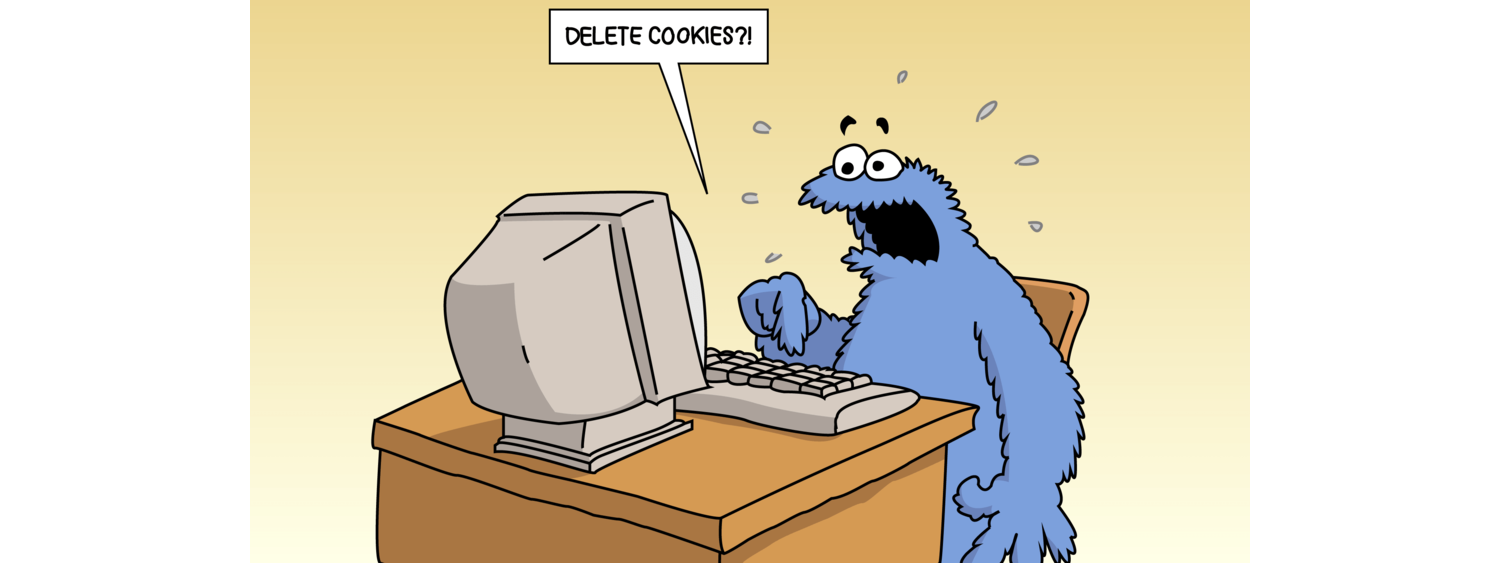
\includegraphics[scale=0.3]{cookie_monster}
\caption*{Before the internet, cookie monster thought he was the only way to get rid of cookies... \#NationalCookieDay}
\end{figure}